\afterpage{\blankpage}
\chapter{Competizioni CTF Attack/Defense}\label{chap:ctfad}
\setcounter{page}{5}

Le competizioni \gls{ctf} di tipo \gls{ad} sono una tipologia di competizioni in cui i partecipanti devono difendere i propri servizi e attaccare i servizi degli avversari, in un contesto di gara estremamente dinamico e competitivo.

In queste competizioni prendono parte diversi team, i quali vengono associati ognuno ad una macchina, solitamente linux, con in esecuzione un insieme di servizi ogniuno dei quali presenta vulnerabilità\footcite{\url{https://faustctf.net/information/attackdefense-for-beginners/}}{faustctf_attackdefense_for_beginners}. I servizi sono accessibili tramite la rete di gara, e sono replicati su tutte le macchine.

\section{Descrizione dell'infrastruttura}

L'infrastruttura di una competizione CTF Attack/Defense è composta da diversi componenti chiave che interagiscono in modo sinergico. Possiamo individuare tre elementi principali che costituiscono l'infrastruttura di gara:
\begin{itemize}
    \setlength{\itemsep}{2pt}
    \setlength{\parskip}{2pt}
    \item Il \textbf{Gameserver}, cuore centrale del sistema che gestisce la competizione
    \item I \textbf{Checker}, responsabili del monitoraggio continuo della rete e dei servizi
    \item Le \textbf{VM dei team}, che ospitano i servizi vulnerabili
\end{itemize}

Il funzionamento di ogniuno di questi componenti è approfondito nei paragrafi successivi, evidenziando inoltre tutte le peculiarità e le funzionalità utili allo svolgimento della competizione.

\subsection{Il Gameserver e i Checker}

Al centro di tutta la competizione c'è il gameserver, entità (che può essere composta da uno o più host) che prende in carico la gestione della competizione eseguento una serie di azioni e fornendo diversi servizi descritti in questo capitolo, essenziali per lo svolgimento della gara stessa.

La competizione è strutturata in tick (o round), ovvero intervalli di tempo in cui ciclicamente il gameserver assegna punti ai team in base alle azioni compiute dagli stessi, e monitora i servizi tramite i checker. Questo tempo può variare da competizione a competizione. I checker sono dei bot che si occupano di supervisionare lo stato della gara eseguendo diverse azioni come:
\begin{itemize}
    \setlength{\itemsep}{2pt}
    \setlength{\parskip}{2pt}
    \item Verificare se il servizio è funzionante e raggiungibile, andando a connettersi ed eseguendo azioni di normale utilizzo, assicurandone anche l'integrità.
    \item Utilizzare il servizio per memorizzare al suo interno una flag, inserita come informazione sensibile normalmente non accessibile seguendo i normali workflow del servizio.
    \item Verificare che le flag inserite nei tick precedenti siano ancora raggiungibili tramite un normale accesso autorizzato, e che pertanto non siano state modificate o rimosse dal team possessore di quella macchina.
\end{itemize}

In generale, rimuovere vecchie flag, avere il servizio non raggiungibile e non avere la possibilità di inserirne di nuove, sono azioni che vanno ad invalidare la normale attività del servizio: il gameserver, rilevate queste problematiche, lo andrà a considerare come totalmente o parzialmente inaccessibile o manomesso, in base alle scelte degli organizzatori.

Si evidenzia come i checker non sfruttino mai le vulnerabilità dei servizi, ma si limitino al loro corretto utilizzo.

\subsection{I servizi, le flag e i flag store}

Ogni flag viene generata e inserita dai checker nel servizio dei vari team ad ogni tick, con una flag sempre differente dalle altre ed ha usualmente una durata massima di valenza (e.g, 5 tick): in questo intervallo di tempo è ancora possibile rubare e consegnare la flag al gameserver ottenendo punti.

Le flag infatti una volta ottenute vanno consegnate al gameserver, che tramite un calcolo che può variare in diverse competizioni, assegna punti al team che l'ha consegnata.

\begin{listing}[H]
\begin{minted}[
    frame=single,
    framerule=0.8pt,
    fontsize=\footnotesize,
    breaklines
]{python}
scale = 15 * sqrt(5) 
norm = ln(ln(5)) / 12 
offense_points[flag] = scale / (1+exp((sqrt(score[attacker][service]) - sqrt(score[victim][service]))*norm))
defense_points[flag] = min(victim_score, offense_points)
\end{minted}
\vspace{-1em}
\caption{Algoritmo di calcolo del valore della flag in CyberChallenge\footciteref{cyberchallenge_ad_rules}}\label{lst:flagcalc}
\end{listing}

Il defense point è il punteggio sottratto al team da cui è stata rubata la flag come parte del punteggio di difesa descritto successivamente.

All'interno della competizione spesso possono esserci dei team di `prova' chiamati \gls{nop} team: questi sono semplicemente macchine non associate a nessun gruppo reale di persone, che offrono i servizi della gara, al solo scopo di renderli usufruibili per eseguire penetration testing. Il loro utilizzo è particolarmente utile ai partecipanti per provare gli attacchi in maniera quanto più fedele e realistica possibile, eseguendo l'attacco su una replica originale del servizio, e non su una potenzialmente soggetta alle modifiche e alle patch del team avversario. Non tutte le competizioni prevedono la presenza dei \gls{nop} team.

Si noti che consegnare le flag del proprio team o quelle appartenenti ai \gls{nop} team non permette di guadagnare nessun punteggio, e ciò è possibile poichè il gameserver ha traccia di tutte le flag, di chi le consegna, e delle macchine in cui sono state originariamente inserite.

Una caratteristica importante da sottolineare riguardo ai servizi di cui si è parlato fino ad ora è che non è sempre vero che per ognuno di essi ci sia una sola flag per tick ed una sola vulnerabilità per singolo tick. Infatti, ogni servizio ha usualmente multiple vulnerabilità e flag per tick al suo interno: i checker che si occupano di inserire le flag potrebbero inserirne diverse, usando diverse parti o impostazioni del servizio.

In caso di servizi con più flag, diremo che questi conterranno diversi flag store. Ciò detto fino ad ora è pertanto valido per ogni flag store, e non per il servizio in generale.

Si noti infine che esiste un set di checker differente per ogni flag store.

\subsection{I Flag ID}

Il gameserver potrebbe rilasciare delle informazioni aggiuntive per ogni flag store, come ad esempio un username, che di per se non va direttamente a permettere l'accesso protetto alla flag, ma da un informazione utile agli attaccanti al fine di poterla individuare più facilmente all'interno del servizio stesso.

Questa informazione aggiuntiva è chiamata Flag ID e viene rilasciata per ogni team, per ogni flag store, e per ogni flag ancora valida nel momento in cui si visita l'\gls{api} esposta dal gameserver, che le espone pubblicamente per tutti i partecipanti. Non è possibile manomettere i Flag ID, in quanto sono informazioni direttamente rilasciate dagli organizzatori, che comunque in assenza di vulnerabilità nei servizi, risultano insufficienti per ottenere flag.

\subsection{Calcolo del punteggio}

A ciascun flag store in gara viene associato un punteggio, che riflette la capacità del team di sfruttare e proteggere le relative vulnerabilità. Il calcolo del punteggio totale si ottiene tradizionalmente mediante una semplice sommatoria dei punteggi parziali.

Il punteggio attribuito a un singolo store è inizialmente determinato da un valore base, soggetto a variazioni durante la competizione in relazione alle prestazioni del team. Tale valore può essere incrementato o ridotto in base a tre componenti aggiuntive:

\begin{itemize}
    \setlength{\itemsep}{2pt}
    \setlength{\parskip}{2pt}
    \item \textbf{Punteggio di \gls{sla}}: misura la disponibilità del servizio, calcolata in proporzione al tempo di effettiva operatività.
    Questo indicatore, generalmente in percentuale, viene applicato al punteggio complessivo dello store. La scelta di attribuirgli un ruolo predominante mira a scoraggiare strategicamente la disattivazione volontaria dei servizi per evitare attacchi, penalizzando severamente tale approccio. Di conseguenza, il mantenimento dell'operatività del servizio (pur nella sua condizione vulnerabile) assume un'importanza critica nella competizione.

    \item \textbf{Punteggio di attacco}: determinato dal numero di invii corretti di flag effettuati dal team. Il valore attribuito a ciascuna flag può variare in funzione della complessità dell'attacco e della tempestività con cui il servizio è stato compromesso rispetto agli altri team.

    \item \textbf{Punteggio di difesa}: tipicamente negativo, poiché quantifica l'inefficacia delle contromisure, è calcolato in base al numero di flag sottratte al team da parte degli avversari. Tale componente tende a controbilanciare, o persino ridurre, il punteggio di attacco relativo allo stesso flag store, potendolo portare anche al di sotto del valore base iniziale. La sua entità è modulata da criteri analoghi a quelli usati per il punteggio di attacco. Per mitigarne gli effetti, risulta essenziale applicare interventi correttivi (\emph{patch}) che impediscano nuovi attacchi, garantendo al contempo la piena operatività del servizio e l'integrità dei dati archiviati (comprese le flag precedenti, la cui perdita comporterebbe un deterioramento del punteggio di \gls{sla}).
\end{itemize}

\begin{listing}[H] 
\begin{minted}[
    frame=single,
    framerule=0.8pt,
    fontsize=\footnotesize,
    breaklines
]{python}
# --- Total score for each service (or better said, flag store) ---
# Service base points 
score[team][service] = 5000 
            
# Sum offensive points 
for flag in stolen_flags[team][service]:
    score[team][service] += offense_points[flag] 
    
# Substract defensive points 
for flag in lost_flags[team][service]: 
    score[team][service] -= defense_points[flag]

# --- Final team score ---
total_score[team] = 0   
for service in services: 
    # Compute SLA of the service
    sla[team][service] = ticks_up[team][service] / ticks[team][service] 
    # Limit scores to 0
    score[team][service] = max(0, score[team][service]) 
    # Add service score
    total_score[team] += score[team][service] * sla[team][service]
\end{minted}
\vspace{-1em}
\caption{Algoritmo di calcolo del punteggio in CyberChallenge\footciteref{cyberchallenge_ad_rules}}\label{lst:scorecalc}
\end{listing}

\begin{figure}[H]
    \centering
    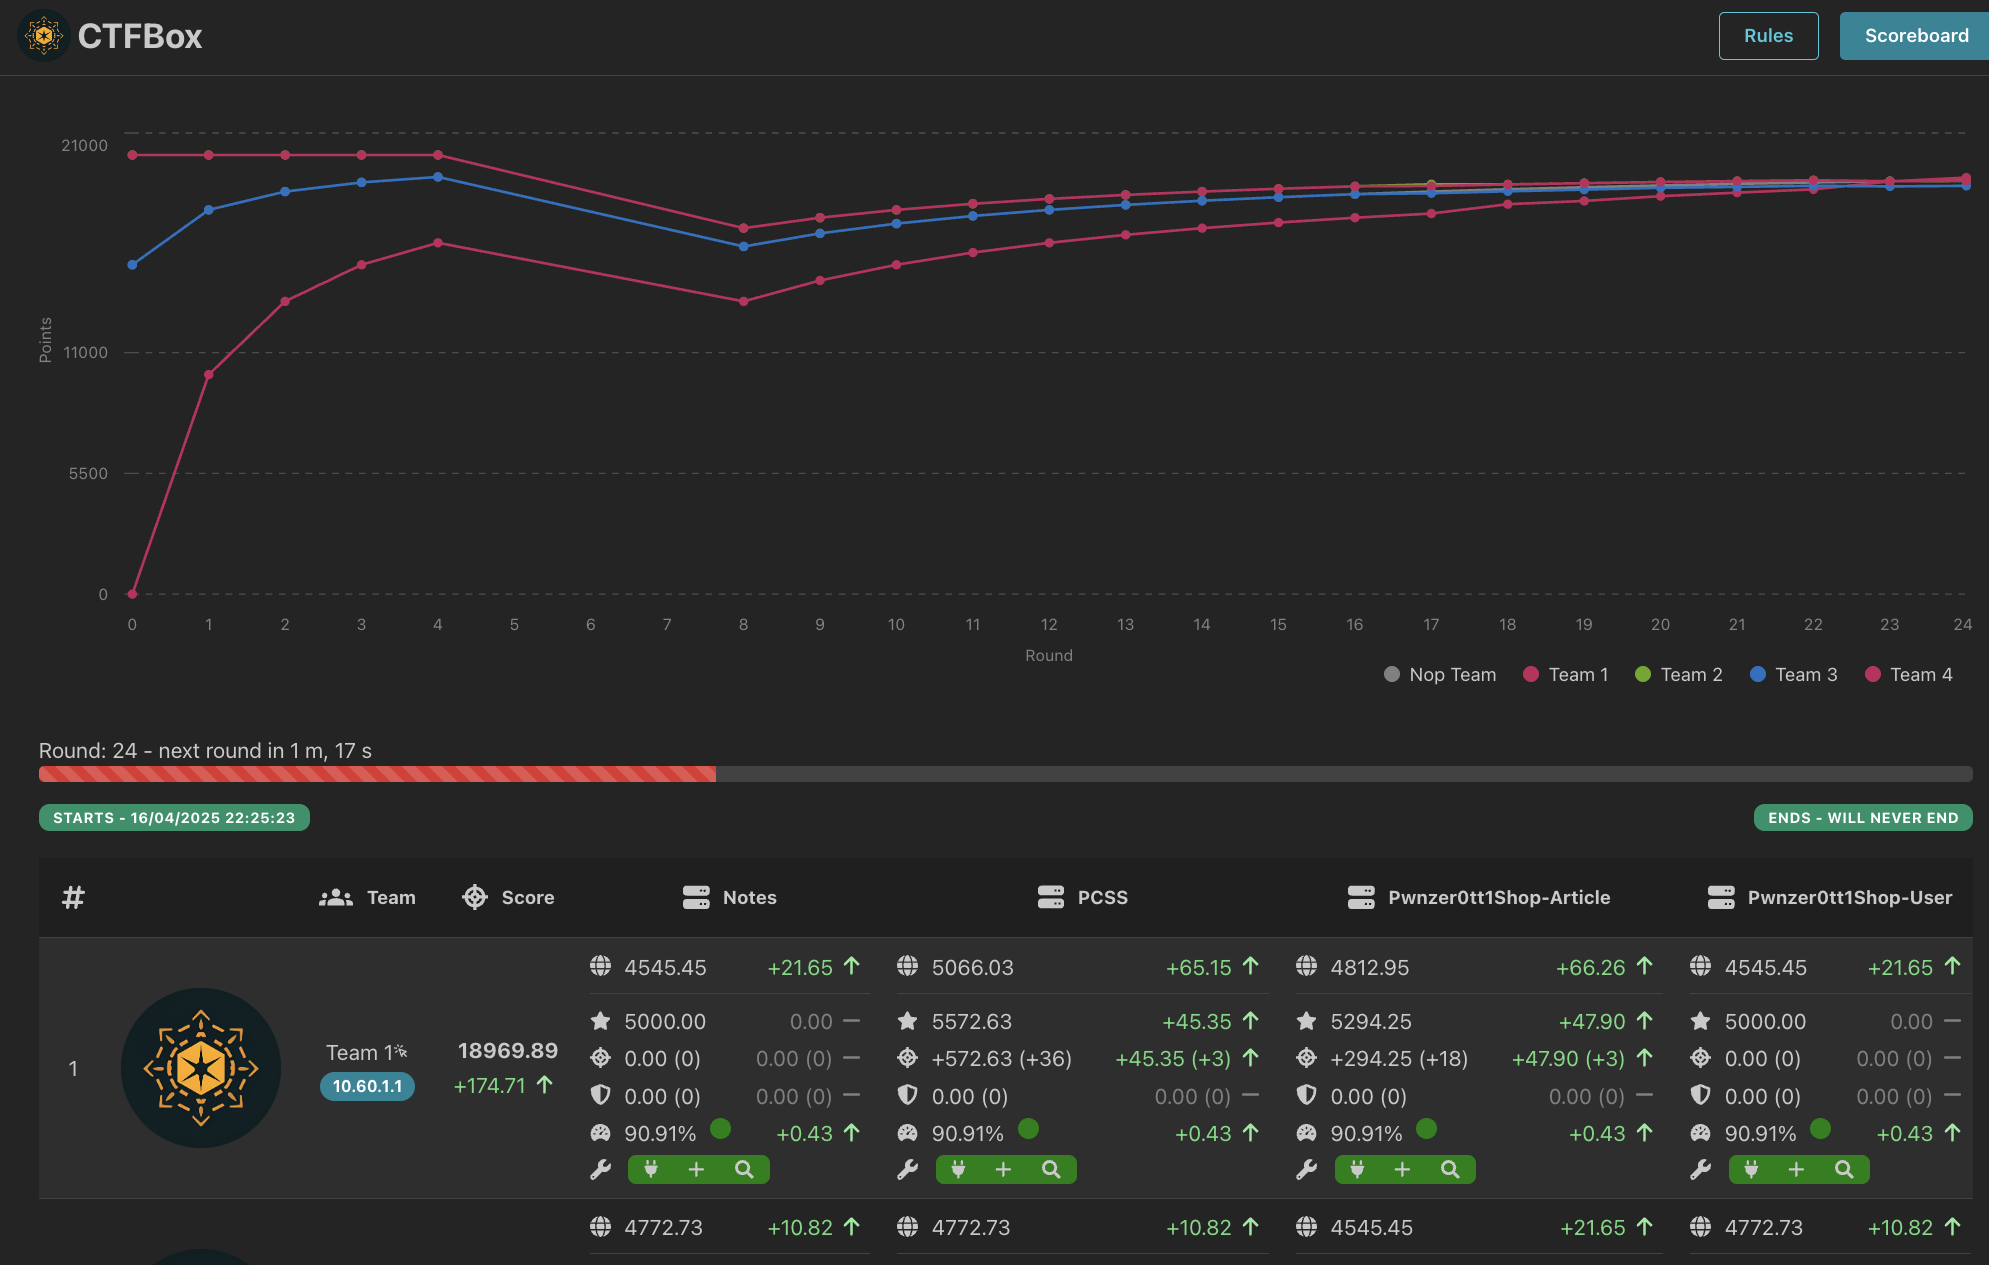
\includegraphics[width=0.98\textwidth]{images/chapter1/ctfbox_scoreboard.png}
    \caption{Scoreboard di una simulazione realizzata con CTFBox\footciteref{ctfbox_gh}}\label{fig:ctfbox_scoreboard}
\end{figure}

\subsection{Rete di gara}

Per questa analisi si prende in considerazione la rete di gara in utilizzo per le competizioni nazionali di Cyberchallenge\footcite{\url{https://ad.cyberchallenge.it/rules/}}{cyberchallenge_ad_rules}, sottolineando come a grandi linee la configurazione di rete è spesso simile, ma potrebbe variare in base alle competizioni e agli organizzatori.

\begin{figure}[H]
    \centering
    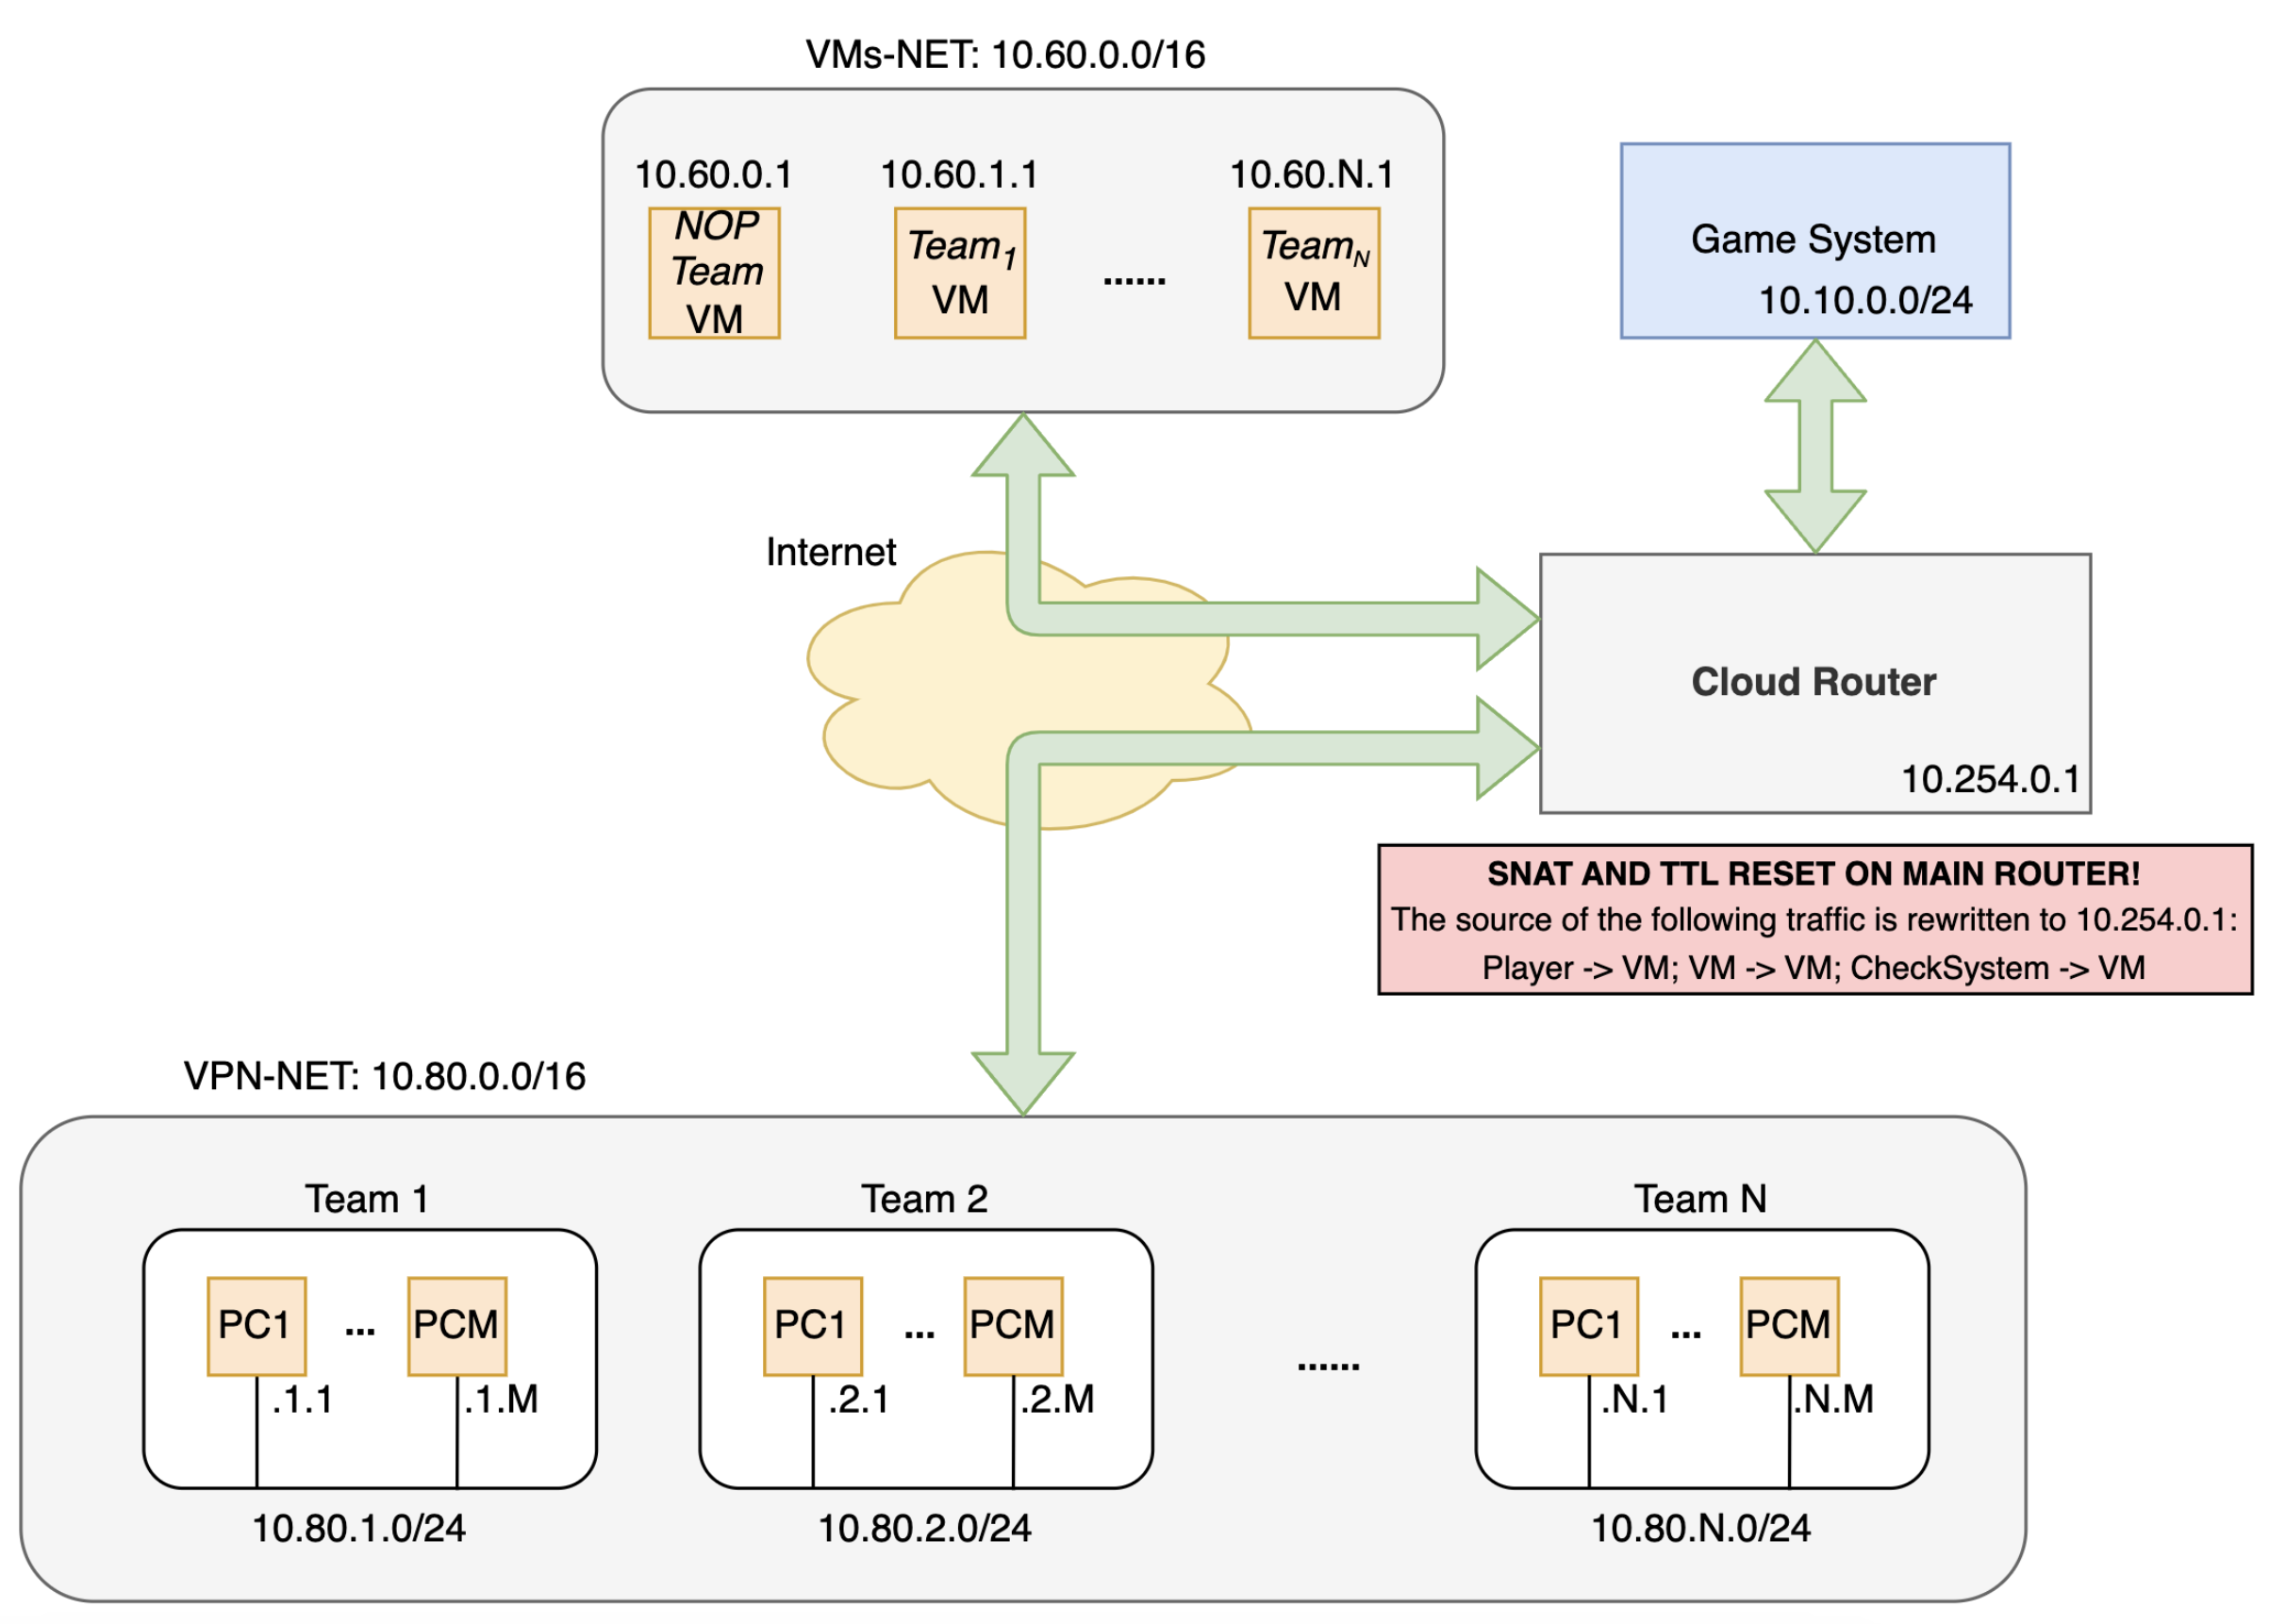
\includegraphics[width=0.8\textwidth]{images/chapter1/ccit_network.png}
    \caption{Modello della rete di gara di Cyberchallenge\footciteref{cyberchallenge_ad_rules}}\label{fig:ccit_network}
\end{figure}

Come si può vedere nella Figura~\ref{fig:ccit_network}, la rete di gara è composta da diversi elementi:
\begin{itemize}
    \setlength{\itemsep}{2pt}
    \setlength{\parskip}{2pt}
    \item La rete dedicata agli organizzatori, dove abbiamo il gameserver (potenzialmente formato da un insieme di host) ed eventuali ulteriori host al servizio degli organizzatori.

    \item La sottorete delle macchine dei team, dove si ha accesso ssh alla propria macchina con i propri servizi vulnerabili.

    \item Una sottorete (spesso realizzata tramite \gls{vpn}) per ogni team, dove sono connessi gli host dei partecipanti con i quali è possibile interagire direttamente con la rete di gara.
\end{itemize}

Al centro di tutto ciò troviamo il cloud router, che si occupa di gestire il traffico in base alle regole imposte dagli organizzatori e in base alla fase in cui si trova la competizione, ma che soprattutto si occupa di anonimizzare il traffico, manipolandolo tramite diverse tecniche tra le quali il \gls{nat}. Tramite il \gls{nat} infatti si nascondono gli indirizzi \gls{ip} delle macchine e dei componenti del team, mascherando nelle richieste la vera identità del mittente con quella del router stesso. Questo è un elemento di fondamentale importanza poichè altrimenti sarebbe davvero molto semplice diversificare le connessioni dei checker da quelle degli attaccanti, andando a perdere l'obiettivo che ha la competizione stessa, ovvero: individuare, sfruttare e difendersi dalle vulnerabilità.

Inoltre si specifica che le reti dei singoli team sono isolate per tutta la competizione al fine di evitare possibili attacchi agli host dei partecipanti, che non sono dei target di interesse nella gara e per cui non è consentita l'esecuzione di attacchi mirati.
Un simile comportamento potrebbe portare alla squalifica del team attaccante a seguito di segnalazioni e analisi del traffico da parte degli organizzatori.

\section{Svolgimento della competizione}

Una competizione \gls{ad} inizia nel momento in cui viene dato accesso alle macchine e alla rete di gara. Usualmente in questa fase c'è un periodo di tempo in cui la rete rimane non accessibile: i team avranno accesso unicamente alle loro macchine, mentre l'accesso ai servizi degli avversari verrà negato. In questo momento tuttavia è già possibile analizzare i servizi, avviare tutti i tool necessari all'avvio degli attacchi, all'analisi della rete, e alla difesa del server (che analizzeremo nel prossimo paragrafo). Finito questo periodo di tempo, la rete di gara viene aperta, e la competizione inizia ufficialmente.

Da ora il gameserver inizia a scandire i tick, i checker iniziano ad utilizzare i servizi e ad inserire le prime flag, pubblicando anche i primi Flag ID.
I team iniziano a lavorare, tentando di difendersi dai primi attacchi, e a loro volta di attaccare rubando le prime flag agli avversari, tutto ciò mantenendo sempre i loro servizi attivi e funzionanti. Ad ogni tick, il gameserver assegna i nuovi punteggi, e i team possono osservare tramite questi dati l'evoluzione della gara stessa, comprendendo quali possono essere le azioni da compiere per massimizzare la crescita del loro punteggio.
Inoltre, viene segnalato pubblicamente quali dei servizi di quale team non sono funzionanti, e perchè sono considerati down: cioè la motivazione per cui i checker hanno segnalato un mal funzionamento.
La competizione termina ad un determinato orario di fine, dove la rete di gara viene chiusa, e il gameserver interrompe l'azione dei checker non accettando, inoltre, nuove submission di flag.

Tutto quello descritto in questo capitolo è possibile simularlo e sperimentarlo tramite il progetto CTFBox\footcite{\url{https://github.com/domysh/ctfbox}}{ctfbox_gh}, nato come fork di Oasis dei TheRomanXpl0it\footcite{\url{https://theromanxpl0.it/about.html}}{theromanxploit} con cui è possibile simulare ma anche svolgere competizioni \gls{ad} di medio-piccole dimensioni in un ambiente realizzato unicamente tramite l'utilizzo di container, con funzionamento e regolamento simile a quello di CyberChallenge\footcite{\url{https://ad.cyberchallenge.it/rules/}}{cyberchallenge_ad_rules}.

\section{Tool utili}

Data l'elevata complessità nello svolgimento di una competizione \gls{ad}, spesso diventa necessario l'utilizzo di tool specializzati che permettano di automatizzare diverse operazioni necessarie durante la gara. Ogni team può sviluppare e utilizare anche tool che facilitano (o perfino che automatizzino) l'attacco e la difesa dei servizi.\\
In generale i tool utilizzati più frequentemente sono quelli descritti di seguito.

\subsection{Traffic Analyzer}

I tool di analisi del traffico permettono di investigare il flusso di dati sulla macchina, in modo da riconoscere e visionare il traffico dei checker e degli attaccanti (anche se anonimizzato). Analizzare il traffico diventa cruciale dal momento in cui un nuovo attacco è attivo sulla rete, poichè permette ai team di analizzarlo, riconoscere la vulnerabilità sfruttata, e intraprendere azioni quanto più immediate per la difesa e la replicazione dello stesso attacco. Normalmente per analizzare il traffico è possibile usare tool tradizionali quali Wireshark\footcite{\url{https://www.wireshark.org/}}{wireshark} o Suricata\footcite{\url{https://suricata.io/}}{suricata}, che tuttavia risultano poco pratici nel loro utilizzo in ambito \gls{ctf} \gls{ad} dove il traffico da analizzare è elevato e continuo. Esistono infatti, tool scritti appositamente per queste competizioni che permettono di analizzarlo in modo più efficiente e veloce, ma anche di riprodurre velocemente gli stessi payload di attacco, come ad esempio Caronte\footcite{\url{https://github.com/eciavatta/caronte}}{caronte} o Tulip\footcite{\url{https://github.com/OpenAttackDefenseTools/tulip}}{tulip}.

Ad esempio Caronte\footciteref{caronte} avvantaggia particolarmente l'analisi del traffico grazie alla sua interfaccia grafica interattiva e di facile utilizzo, che permette di visualizzare i flussi di traffico \gls{tcp} aggregati e decodificati in pochissimi click, e permettendone anche il tagging tramite l'utilizzo di \gls{regex} personalizzate, che permettono ad esempio di identificare una flag in uscita (quindi rubata o controllata dal checker) e le flag in entrata (quindi le nuove flag inserite dal gameserver). Ogni connessione è classificata tramite tag e colori personalizzabili in base alla porta di destinazione (e.g.\ \gls{http}:\ blu, SSH:\ verde), permettendo una mappatura visiva immediata dei servizi sotto attacco. Inoltre include una timeline interattiva, campionata al minuto per scorrere la porzione di traffico che si desidera analizzare.

\begin{figure}[H]
    \centering
    
\includegraphics[width=0.13\textwidth]{images/chapter1/CaronteLogo.png}
    \caption{Logo di caronte}\label{fig:caronte_logo}
\end{figure}

\begin{figure}[H]
    \centering
    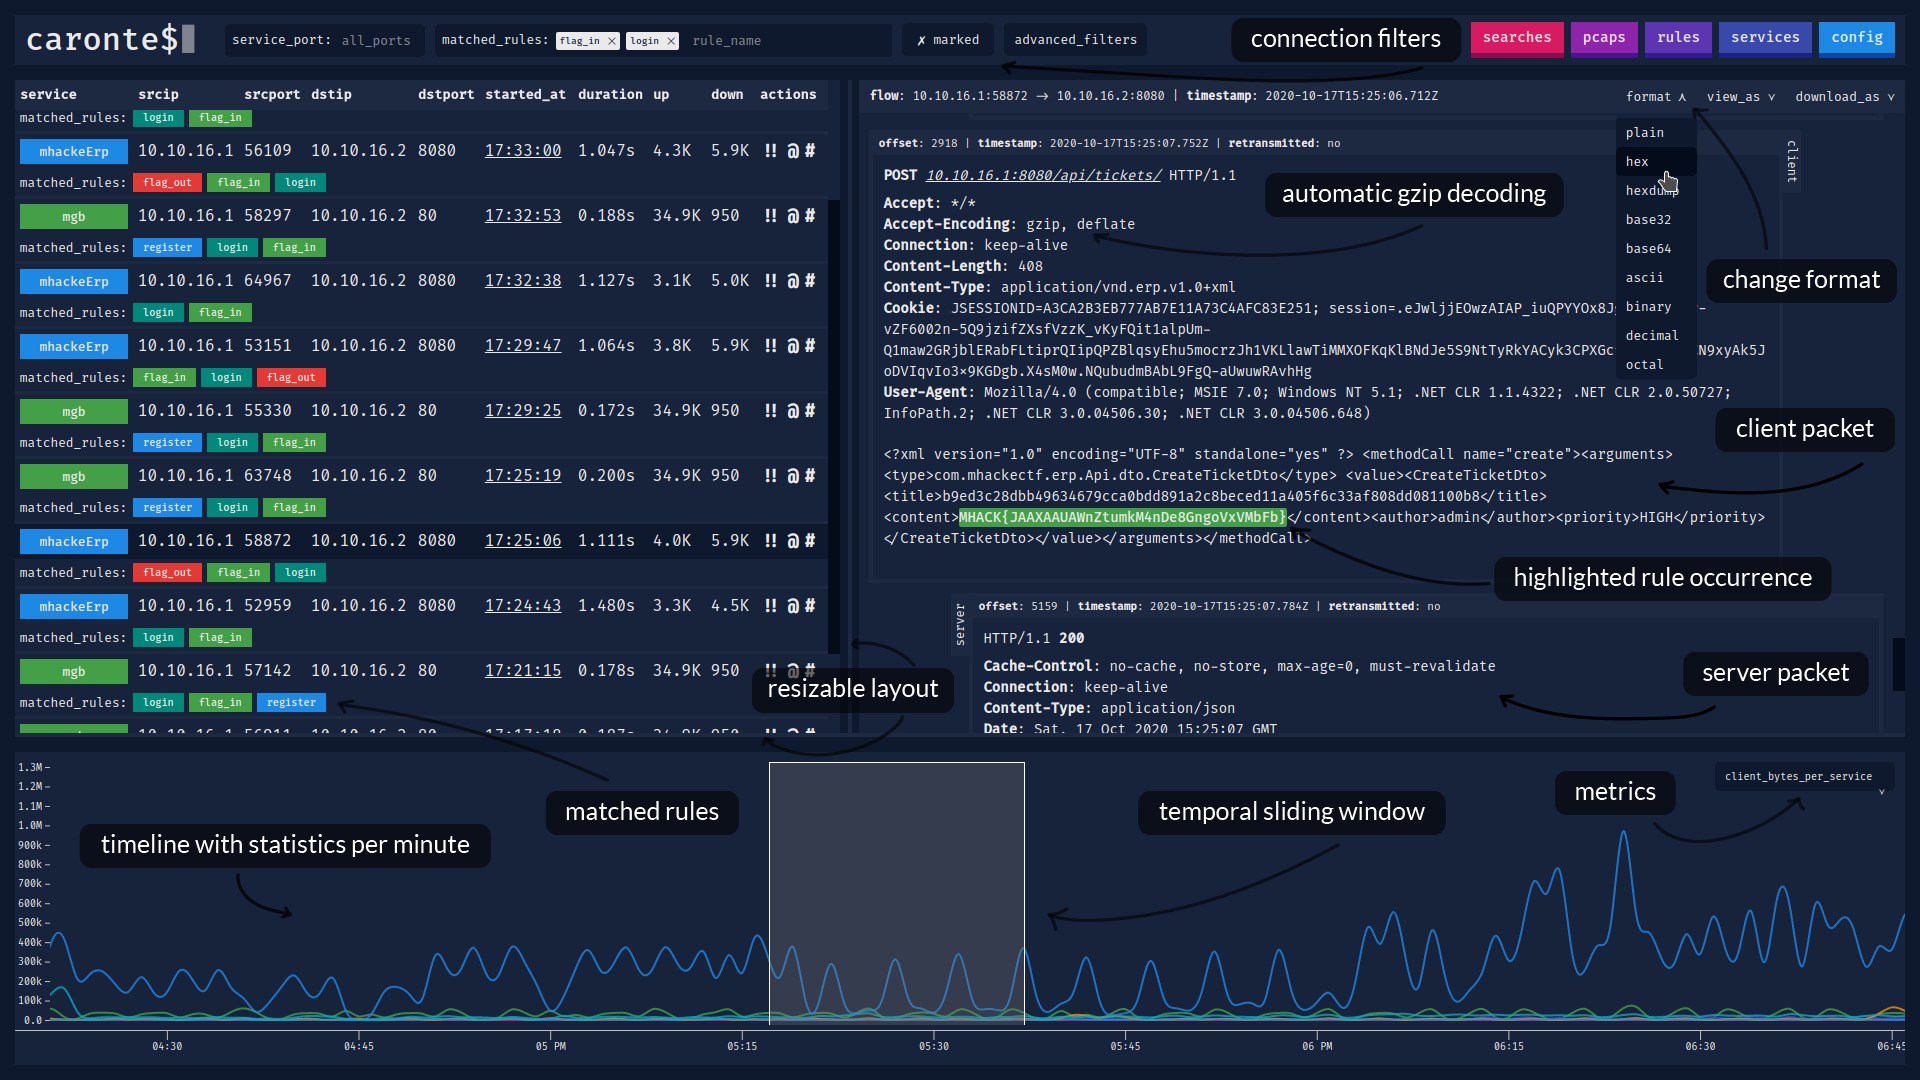
\includegraphics[width=0.98\textwidth]{images/chapter1/caronte_interface.png}
    \caption{Interfaccia di Caronte}\label{fig:caronte_interface}
\end{figure}

\subsection{Attacker \& Submitter}

Gli strumenti di attacco e submission automatizzati coordinano gli attacchi, assistono nella scrittura degli exploit e ne monitorano l'esecuzione, programmandola e parallelizzandola. Questi tool sono fondamentali per permettere all'attaccante di concentrarsi sulla progettazione del singolo attacco, anziché sulla gestione della sua esecuzione su tutte le macchine nemiche. Inoltre, grazie alla tracciabilità degli attacchi, è possibile identificare problemi durante l'esecuzione e monitorare quali team iniziano a difendere i propri servizi. Solitamente (ma non sempre) questi strumenti gestiscono anche la submission delle flag al gameserver in modo centralizzato, semplificando il rispetto delle regole organizzative che limitano frequenza e quantità per prevenire attacchi bruteforce o DoS all'infrastruttura.

Esempi di tali tool includono DestructiveFarm\footciteref{destructivefarm}, che presenta tuttavia criticità nell'analisi dell'andamento degli attacchi, e ExploitFarm\footciteref{exploitfarm}, sviluppato proprio per ovviare a queste limitazioni. A differenza di DestructiveFarm\footciteref{destructivefarm}, ExploitFarm\footciteref{exploitfarm} offre un coordinamento più efficiente degli attacchi, un monitoraggio avanzato e una schedulazione semplificata, supportando attacchi distribuiti su più macchine con funzionalità di analisi in tempo reale.

La sua infrastruttura ricalca quella di DestructiveFarm\footciteref{destructivefarm}: un server centrale gestisce gli exploit e le submission, mentre client distribuiti eseguono gli attacchi e inviano le flag al server, bilanciando il carico computazionale derivante dalla replicazione degli exploit. Il sistema include un client terminale per l'esecuzione degli attacchi e un'interfaccia web centralizzata per il monitoraggio e l'analisi. La piattaforma è orientata alla raccolta dati e alla reportistica, con funzionalità di versioning degli exploit, registrazione dettagliata di ogni esecuzione e analisi delle cause di fallimento per ottimizzare gli attacchi.

La dinamicità del sistema consente modifiche in real-time, propagate immediatamente all'intera infrastruttura, e notifiche automatiche per criticità o errori rilevati durante le operazioni.

\begin{figure}[H]
    \centering
    
\includegraphics[width=0.13\textwidth]{images/chapter1/ExploitFarmLogo.png}
    \caption{Logo di ExploitFarm}\label{fig:exploitfarm}
\end{figure}

\begin{figure}[H]
    \centering
    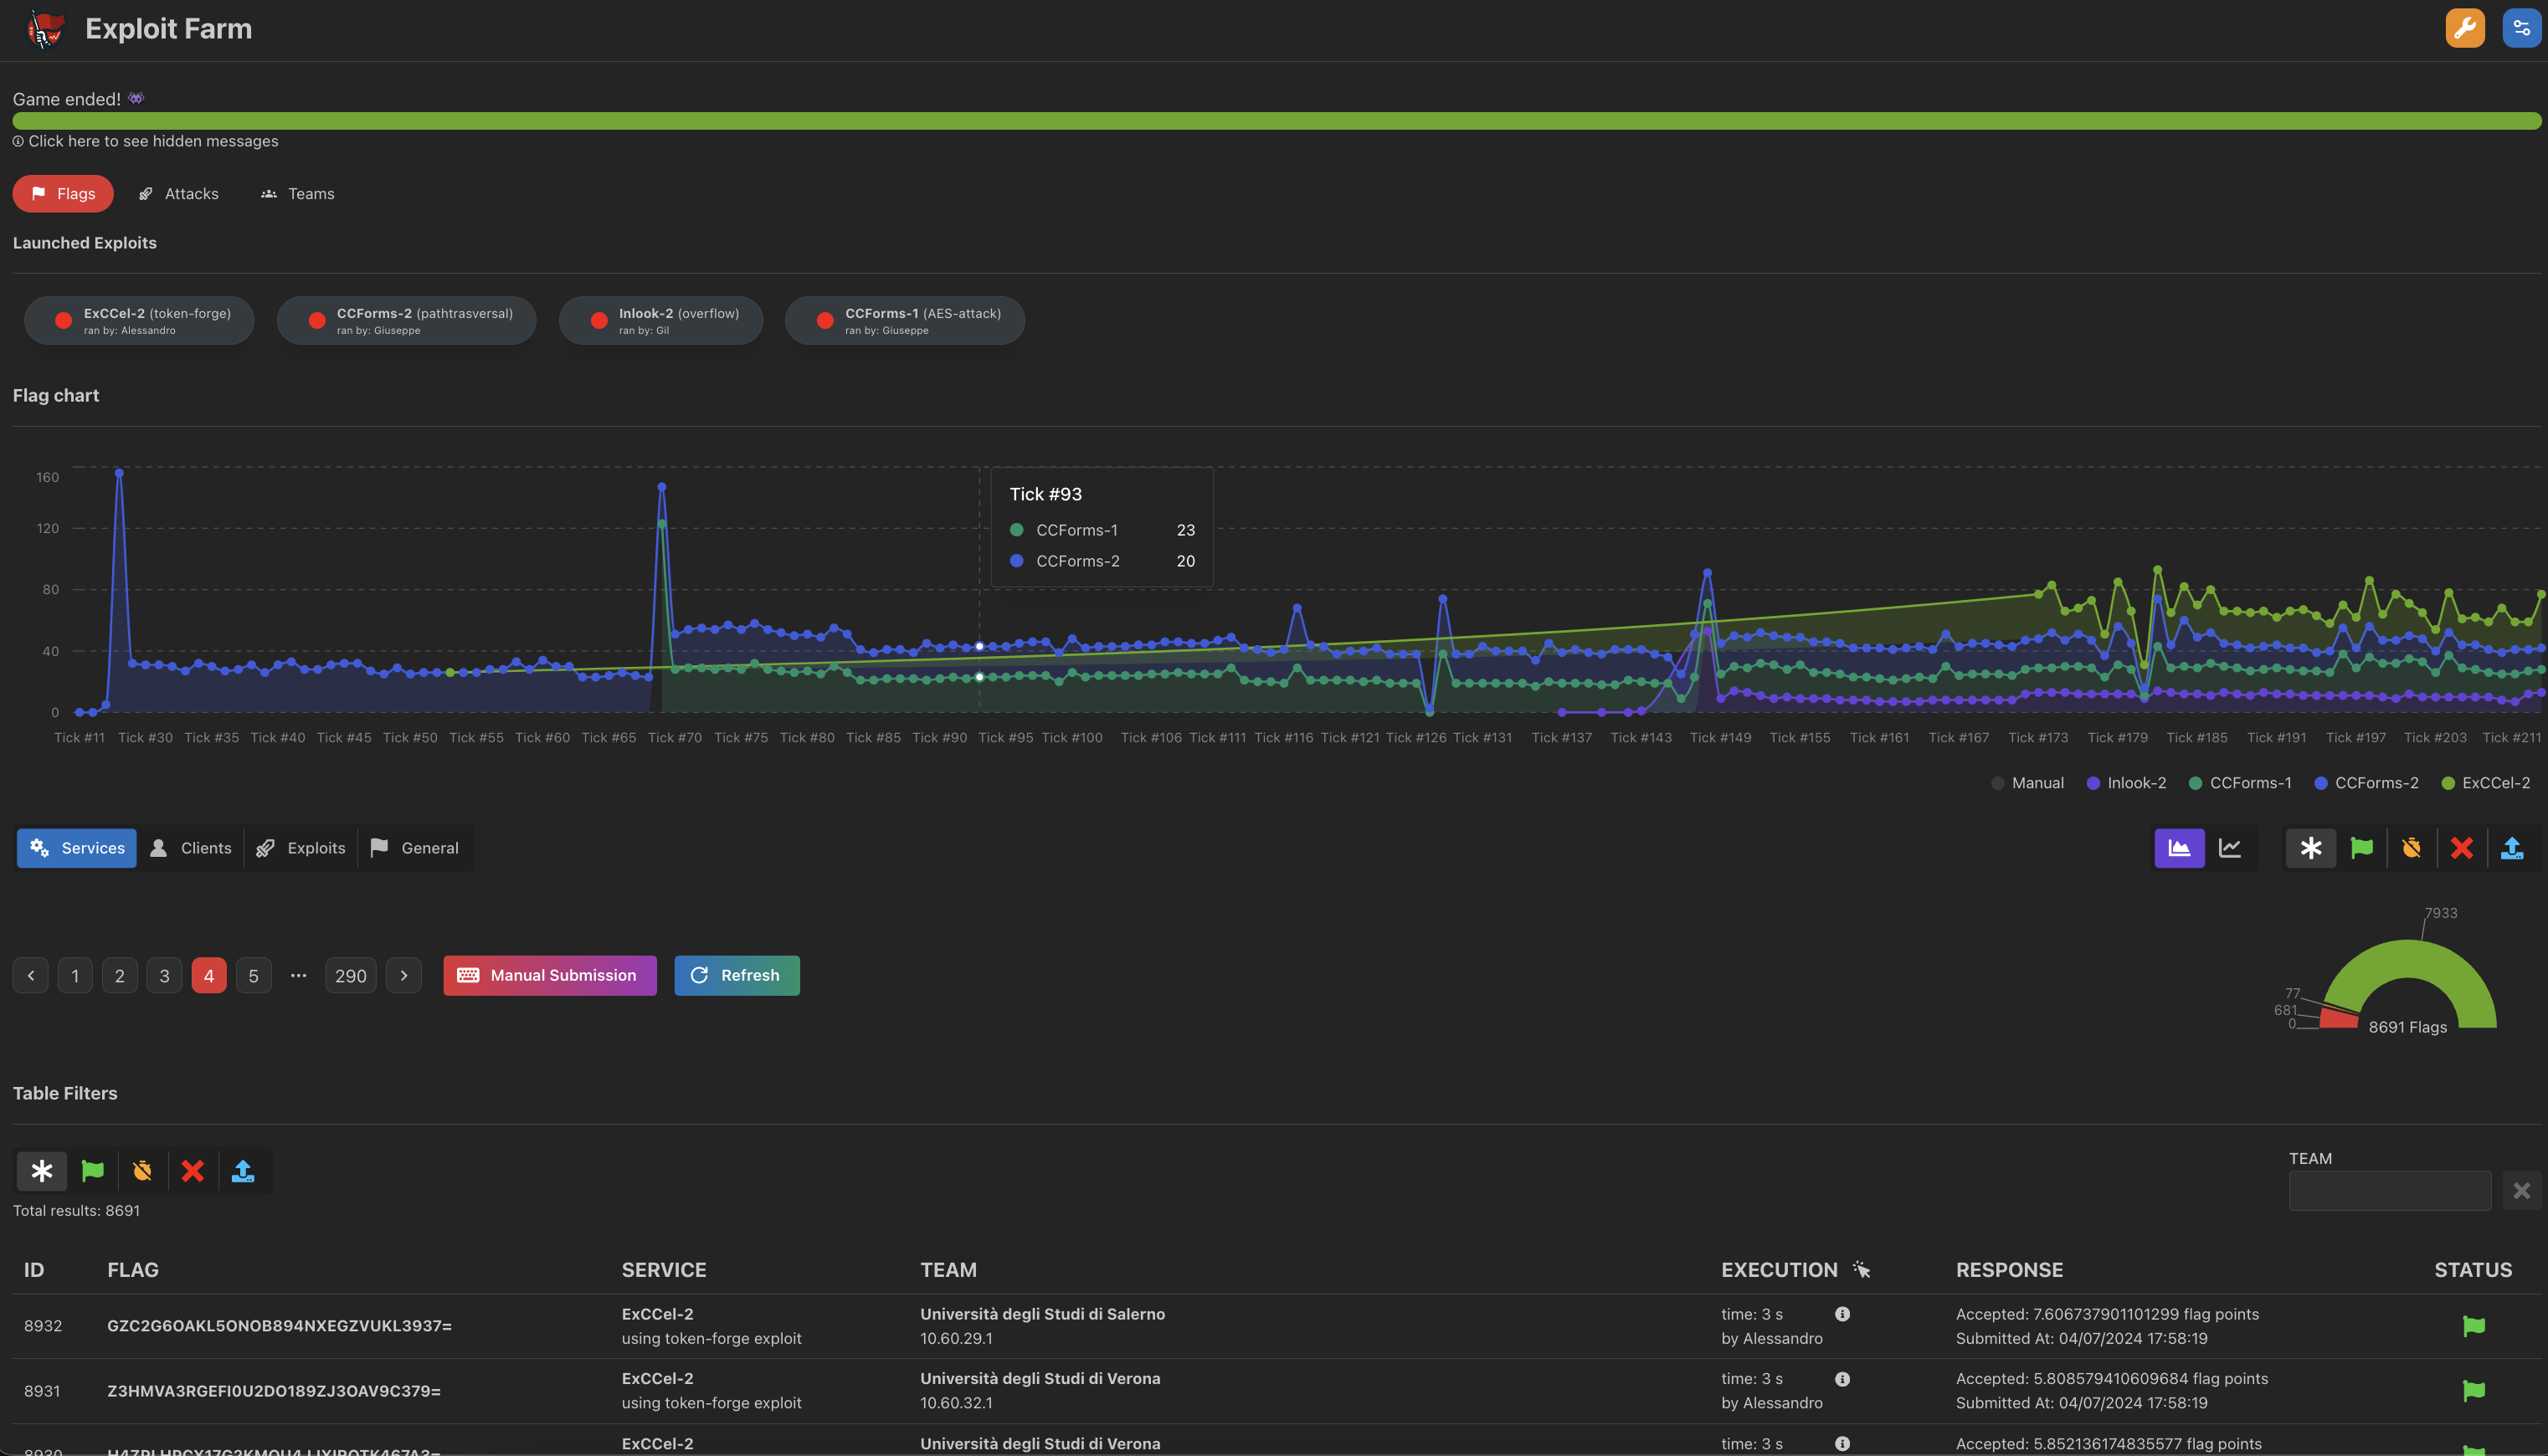
\includegraphics[width=0.98\textwidth]{images/chapter1/exploitfarm_interface.png}
    \caption{Interfaccia di ExploitFarm}\label{fig:exploitfarm_interface}
\end{figure}

\subsection{Proxy e Firewall}

Questi tool permettono di filtrare il traffico in modo da riconoscere e bloccare gli attacchi. Questi tool possono essere molto utili nella difesa, e permettono di bloccare gli attacchi senza di fatto eseguire una modifica sui servizi stessi, spesso diretta conseguenza di malfunzionamenti per errori eseguiti durante questa fase. Questo modo di proteggere i servizi, tuttavia, risulta spesso incompleto e superabile, ma se ben progettato e correttamente utilizzato può essere un'ottima soluzione temporanea, se non una soluzione completa in alcune casistiche specifiche. Spesso però la soluzione più efficace rimane comunque quella di correggere la vulnerabilità. Tool di questo genere sono ad esempio \gls{ctf} Proxy\footcite{\url{https://github.com/ByteLeMani/ctf_proxy}}{ctf_proxy} o il tool di cui tratta questa tesi Firegex\footcite{\url{https://github.com/Pwnzer0tt1/firegex}}{firegex_gh}.

\begin{figure}[H]
    \centering
    
\includegraphics[width=0.13\textwidth]{images/chapter1/FiregexLogo.png}
    \caption{Logo di Firegex}\label{fig:firegex_logo}
\end{figure}

\section{Esempio di un servizio vulnerabile: PCSS}

Consideriamo come esempio un servizio vulnerabile presente nel simulatore di competizioni \gls{ad} CTFBox\footcite{\url{https://github.com/domysh/ctfbox}}{ctfbox_gh}, denominato PCSS (Permanent Cat Storage Service).

Il servizio è composto da un semplice file python e permette di memorizzare e leggere dei testi tramite una connessione \gls{tcp} attraverso un'interfaccia \gls{cli} molto semplice. Il servizio presenta un solo flag store, ma ha al suo interno due vulnerabilità, pertanto per renderlo sicuro è necessario correggerle entrambe.

La registrazione al servizio avviene in modo anonimo: selezionando la funzione di creazione del database, il servizio fornisce un id alfanumerico del database, e un token jwt di accesso con cui è possibile accedere al medesimo in seguito.

Una volta registrati, o eseguito l'accesso tramite il token, è possibile elencare i file presenti nel database, leggerne il contenuto, e crearne nuovi.

\begin{listing}[H] 
\begin{minted}[
    frame=single,
    framerule=0.8pt,
    fontsize=\footnotesize,
    breaklines
]{bash}
PCSS - Permanent Cat Storage Service

          /\_/\
         ( o.o )  
          > ^ <
      __/_______\__
     |             |
     |   WELCOME   |
     |_____________|

Meow! I'm a cat and I'm here to help you store your files.
A way more secure, reliable and fun way to store your files.

--------------------------------------------------
1. Create a new database
2. Access an existing database
3. Exit

Insert your choice:
\end{minted}
\vspace{-1em}
\caption{Interfaccia CLI di PCSS (da CTFBox\footciteref{ctfbox_gh})}\label{lst:pcss_interface}
\end{listing}

A livello tecnico il servizio crea una cartella per ogni database, e all'interno di essa crea i file richiesti.

Il gameserver pubblica come Flag ID l'id del database in cui si trova la flag, e il nome del file in cui è memorizzata.

Come è possibile notare, i flag id non sono sufficienti per accedere alla flag, ma sono un'informazione utile per gli attaccanti per individuare più facilmente la flag all'interno del servizio, e inoltre ci è di aiuto per comprendere dove il servizio memorizza le flag, in questo caso in un file nel database.

La prima vulnerabilità che possiamo individuare è una vulnerabilità di \gls{lfi}:

\begin{listing}[H] 
\begin{minted}[
    frame=single,
    framerule=0.8pt,
    fontsize=\footnotesize,
    breaklines
]{python}
def read_file():
    file = input("Please insert the file name: ").strip()
    print("File content:")
    subprocess.run(["cat", f"./data/{ctx.loggined_db}/{file}"])
    print("")
\end{minted}
\vspace{-1em}
\caption{Funzione vulnerabile a Local File Inclusion nel servizio PCSS (da CTFBox\footciteref{ctfbox_gh})}\label{lst:scorecalc}
\end{listing}

Inserendo semplicemente \texttt{`../<database\_id>/<file\_name>'} come nome del file, è possibile accedere a file esterni al database, e quindi anche alla flag.

La seconda vulnerabilità invece è una vulnerabilità di natura crittografica causata dall'uso di una vecchia versione della libreria \texttt{jwt} (versione 0.5.4), che permette di inserire nel token come algoritmo di firma \texttt{none} e quindi di bypassare la verifica della firma, permettendo di generare un token malevolo per accedere al database.

Questo è possibile poichè la prima parte del token \gls{jwt} è in chiaro, e la sua autenticità non è garantita, per cui è usualmente buona pratica specificare lato server quali algoritmi di firma sono supportati, escludendo attacchi di questo tipo. Questa vulnerabilità è la medesima riscontrata in un famoso framework di autenticazione \gls{jwt} in NodeJS e classificata come CVE-2022-23540\footcite{\url{https://nvd.nist.gov/vuln/detail/cve-2022-23540}}{cve_2022_23540}.

È pertanto possibile costruire un token \gls{jwt} valido per accedere al database, e quindi alla flag, senza conoscere il segreto di firma:

\begin{listing}[H]
\begin{minted}[
    frame=single,
    framerule=0.8pt,
    fontsize=\footnotesize,
    breaklines
]{python}
def attack(team_ip: str, flag_id):
    #The bugged jwt is encoded manually but you could also use a jwt lib to make it
    first_part = base64.b64encode(json.dumps({"alg": "none", "typ": "JWT"}).encode()).decode().replace("=", "")
    data_part = base64.b64encode(json.dumps({'db': flag_id['db_name']}).encode()).decode().replace("=", "")
    jwt = f"{first_part}.{data_part}."
    conn = CatStorage(team_ip)
    conn.login(jwt)
    result = conn.read_file(flag_id["filename"])
    conn.close()
    return result
\end{minted}
\vspace{-1em}
\caption{Funzione per eseguire un attacco tramite un token JWT malevolo su PCSS (da CTFBox\footciteref{ctfbox_gh})}\label{lst:scorecalc}
\end{listing}

La difesa di questo servizio è piuttosto semplice, ma potrebbe risultare anche facilmente soggetta ad errori che potrebbero comprometterne il funzionamento: ciò potrebbe essere causato dall'aggiornamento della libreria \texttt{jwt} che se soggetta a cambiamenti alle sue \gls{api} nelle versioni successive, potrebbe portare a malfunzionamenti imprevisti del servizio stesso, e quindi necessitare di ulteriori modifiche al servizio.

In alternativa potremmo utilizzare sistemi come firegex\footcite{\url{https://github.com/pwnzer0tt1/firegex}}{firegex_gh} che tramite la sua nuova funzione \gls{nfproxy} può eseguire la decodifica del token \gls{jwt} per verificare che l'algoritmo nel token sia quello previsto dal servizio, interrompendo i tentativi di accesso malevoli. Inoltre filtrando anche i doppi punti nel traffico \gls{tcp} in ingresso, possiamo protteggere il servizio anche dalla vulnerabilità di \gls{lfi}.